\documentclass[answers,12pt,addpoints]{exam}
\usepackage{graphicx,multicol}
\usepackage{charter,amsmath,amssymb}
\usepackage{eulervm}
\usepackage[letterpaper,margin=1in]{geometry}
\pagestyle{headandfoot}
\runningheadrule
\runningheader{\bf Math 265}
{\bf Exam Three, Page \thepage\ of \numpages}
{\bf 10 April 2015}
\firstpagefooter{}{}{}
\runningfooter{}{}{}
\let\cos\relax\DeclareMathOperator{\cos}{\mathsf{cos}}
\let\sin\relax\DeclareMathOperator{\sin}{\mathsf{sin}}
\let\ln\relax\DeclareMathOperator{\ln}{\mathsf{ln}}
\let\lim\relax\DeclareMathOperator*{\lim}{\mathsf{lim}}
\everymath{\displaystyle}
\begin{document}
\begin{center}
\huge Math 265 Exam Three\\
\LARGE Spring 2015
\end{center}

\ifprintanswers\else
\begin{center}
\fbox{\fbox{\parbox{5.5in}{
This exam has \numquestions~questions.
It has been printed on \numpages~pages and is worth \numpoints~points.
Answer all the questions in the spaces provided.
%The last page has been left blank for your calculations.
Although you may use any calculator on this exam,
you must clearly indicate how you arrived at your answers
in order to receive maximum credit.
By signing below, you pledge that you
\begin{enumerate}
\item will not communicate to any person in any conceivable way anything
about the contents of this exam
until all students have taken it, and
\item have not been the recipient of such communication from anyone else.
\end{enumerate}}}}
\end{center}
\vspace{.2in}
\makebox[\textwidth]{Your signature:\enspace\hrulefill}\\
\vspace{.2in}\\
\makebox[\textwidth]{Your name:\enspace\hrulefill}\\
\begin{center}\gradetable[h][questions]\end{center}
\fi

\begin{questions}

\question[25] Evaluate the integral
$\int_0^1\int_{e^y}^e\frac{x}{\ln{x}}dxdy$.
\begin{solution}
Changing the order of integration gives
\[\int_1^e\int_0^{\ln{x}}\frac{x}{\ln{x}}dydx
=\int_1^e\left.\frac{xy}{\ln{x}}\right|_0^{\ln{x}}dx
=\int_1^ex\;dx=\left.\frac{x^2}{2}\right|_1^e
=\frac{e^2-1}{2}\]
\end{solution}

\begin{multicols}{2}
\question[25] Calculate $\int_R\sqrt{x^2+y^2}\;dA$ where $R$
is the annular region shown at the right.
\begin{center}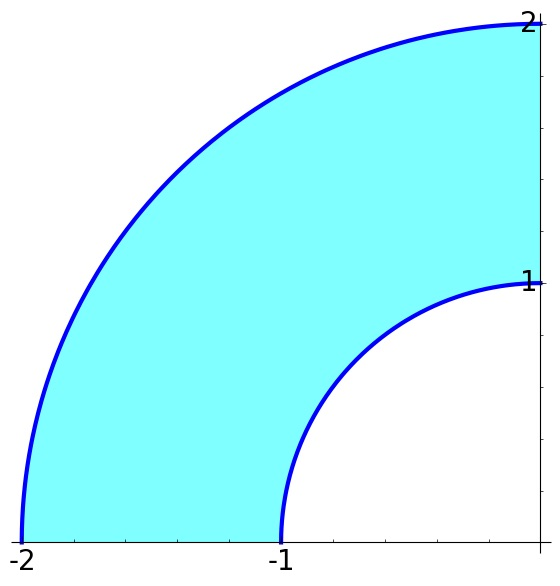
\includegraphics[scale=.25]{WasherWedge}\end{center}
\end{multicols}

%\question[25] Evaluate the integral
%$\int_0^1\int_0^{\sqrt{1-x^2}}\int_0^{\sqrt{x^2+y^2}}
%\frac{dzdydx}{\left(x^2+y^2+z^2\right)^2}$.

\begin{multicols}{2}
\question[25] A cube of side length 2 is composed
of two materials, seperated by a plane slanting down
from the top corner to cut the bottom face in a diagonal,
as shown at the right. The material above the plane
has density $\delta\left(x,y,z\right)$ and the material
above the plane has density $\epsilon\left(x,y,z\right)$,
both measured in $\mathsf{gm}/\mathsf{m}^3$.
Write down an interated integral to find the mass of the cube.
\begin{center}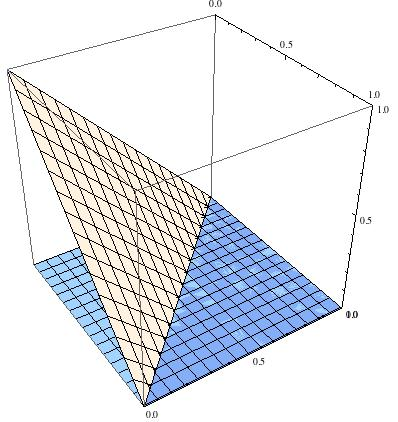
\includegraphics[scale=.4]{BoxPlane}\end{center}
\end{multicols}

\question[25] 
\begin{parts}
\begin{multicols}{2}
\part\label{CirclePart} Find the points of intersection of
the circle of radius~$\sqrt{2}$ centered at the
origin and the circle of radius~1 centered at the point
$\left(0,1\right)$. These circles are shown at the right.
\begin{center}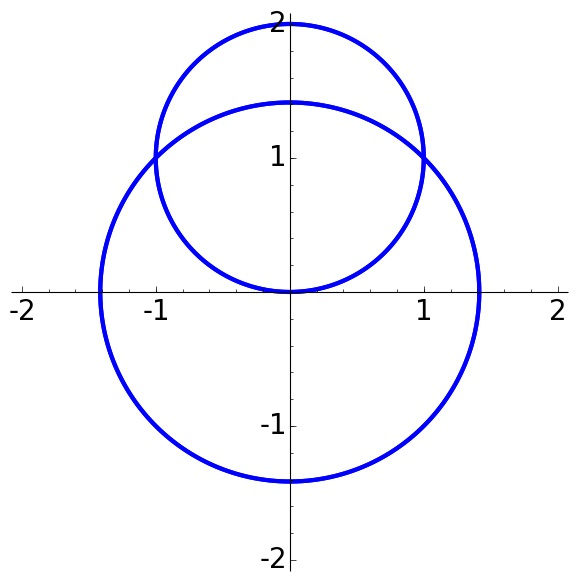
\includegraphics[scale=.25]{TwoCircles}\end{center}
\end{multicols}
\begin{solution}[1in]
Substituting $x^2=-y^2$ into $x^2+\left(y-1\right)^2=1$
gives
\begin{align*}
2-y^2+\left(y-1\right)^2=1\\
\implies\qquad 2-y^2+y^2-2y+1=1\\
\implies\qquad 2-2y=0
\end{align*}
so $y=1$. Substituting $y=1$ into $x^2+y^2=2$ gives $x=\pm 1$.
It follows that the points of intersection are $\left(-1,1\right)$
and $\left(1,1\right)$.
\end{solution}
\part\label{FirstSphere}
Find an equation in spherical coordinates for the sphere
of radius~1 centered at the point $\left(0,0,1\right)$.
\begin{solution}[1in]
The rectangular equation is $x^2+y^2+\left(z-1\right)^2=1$.
Substituting $x=\rho\sin{\phi}\cos{\theta}$,
$y=\rho\sin{\phi}{\sin{\theta}}$, $z=\rho\cos{\phi}$ gives
\begin{align*}
1&=\rho^2\sin^2{\phi}\cos^2{\theta}
+\rho^2\sin^2{\phi}\sin^2{\theta}+\left(\rho\cos{\phi}-1\right)^2\\
&=\rho^2\sin^{\phi}+\rho^2\cos^2{\phi}-2\rho\cos{\phi}+1\\
&=\rho^2-2\rho\cos{\phi}+1
\end{align*}
so that $\rho=2\cos{\phi}$.
\end{solution}
\part Write down, but do not evaluate, an iterated integral
to find the volume of the region inside the sphere in (\ref{FirstSphere})
but outside the sphere of radius~$\sqrt{2}$ centered at the origin.
\begin{solution}[1in]
By (\ref{CirclePart}) the two spheres meet in the circle
$\rho=\sqrt{2},\phi=\frac{\pi}{4}$. So the volume is given by
\[\int_0^{2\pi}\int_0^{\pi/4}\int_{\sqrt{2}}^{2\cos{\phi}}
\rho^2\sin{\phi}d\rho d\phi d\theta.\]
\end{solution}
\end{parts}

\end{questions}
\end{document}
